%% The first command in your LaTeX source must be the \documentclass command.
%%
%% Options:
%% twocolumn : Two column layout.
%% hf: enable header and footer.
\documentclass[
% twocolumn,
% hf,
]{ceurart}

%%
%% One can fix some overfulls
\sloppy
\usepackage{graphicx}
\usepackage{textgreek}
\usepackage{enumitem}
%%
%% Minted listings support 
%% Need pygment <http://pygments.org/> <http://pypi.python.org/pypi/Pygments>
\usepackage{listings}
%% auto break lines
\lstset{breaklines=true}

%%
%% end of the preamble, start of the body of the document source.
\begin{document}

%%
%% Rights management information.
%% CC-BY is default license.
\copyrightyear{2025}
\copyrightclause{Copyright for this paper by its authors.
  Use permitted under Creative Commons License Attribution 4.0
  International (CC BY 4.0).}

%%
%% This command is for the conference information
\conference{OCL 2025 at STAF 2025,
 10 - 13 June 2025 Koblenz, Germany}

%%
%% The "title" command
\title{OCL Collection Optimization - Part 3 - Cascades}

%%
%% The "author" command and its associated commands are used to define
%% the authors and their affiliations.
\author[1,2]{Edward D. Willink}[%
orcid=0000-0003-3124-4019,
email=ed@willink.me.uk,
]
\cormark[1]
\fnmark[1]
\address[1]{Willink Transformations Ltd, Reading England}
\address[2]{Eclipse Foundation}



%%
%% The abstract is a short summary of the work to be presented in the
%% article.
\begin{abstract}
Collections and iterations provide much of the power of OCL. The specification of the OCL Standard Library as operations and and iterations encourages implementation and execution using building blocks. We identify how this approach leads to inefficient execution. We show how providing a sounder formality for iterations and restructuring collections with co-collections enables functionality to be shared across cascades of collection operations.
\end{abstract}

%%
%% Keywords. The author(s) should pick words that accurately describe
%% the work being presented. Separate the keywords with commas.
\begin{keywords}
  OCL\sep
  Collection optimization \sep
  Iteration optimization
\end{keywords}

%%
%% This command processes the author and affiliation and title
%% information and builds the first part of the formatted document.
\maketitle

\section{Introduction}

OCL \cite{OCL-2.4} evolved to satisfy UML's need for textual model constraints where graphics was not appropriate. Unfortunately early tooling was either of insufficient quality or not used and so the OCL constraints that formed part of UML models prior to UML 2.5 contained hundreds of errors.

For UML 2.5 \cite{UML-2.5}, Eclipse OCL \cite{Eclipse-OCL} was used to remove all syntactical errors such as mismatched parentheses or the use of the OCL 1 Enumeration Literal syntax. Nearly all semantic errors such as inappropriate operators or operations were also resolved. No assessment of the functional appropriateness of the constraints was made.

During development of Eclipse OCL's Validity View, UML's OCL constraints were accidentally used directly on the UML metamodel. Execution at least started, but took far too long to make any useful observations of the utility of the constraints. Investigation of the unacceptable speed diagnosed that long cascades of collection operations contributed to very high order execution times. The manual transcriptions and caches of real UML tools avoid the high orders. Automated OCL tooling clearly needs improving to emulate what manual implementations do. But how? Finally inspiration struck.

In this paper we briefly review the collection innovations from part 2 \cite{Willink-Collections2}. In Section~\ref{Cascade Execution} we examine the traditional execution flow for a simple example and discuss its limitations and the remedy that a \verb!gather!-\verb!gather! optimization offers. In Section~\ref{Idioms} we identify some idiomatic usages in the UML's OCL; one is resolved by a \verb!gather!-\verb!gather! optimization. The other motivates a \verb!gather!-\verb!search! optimization that we discuss in Section~\ref{gather-search-optimization}. In Section~\ref{Results} we present results that show the potential benefits of the  \verb!gather!-\verb!gather! optimization. Then we discuss Further Work in Section~\ref{Further Work} and Related Work in Section~\ref{Related Work}. Finally we conclude in Section~\ref{Summary}.

In part 2, we proposed to replace the implementation (but not specification) of the four collection kinds by a single basic sequence with an optional CoCollection in which support for the set and bag aspects could be lazily computed, cached and shared. We also proposed new declarative \verb!gather! and procedural \verb!search! iterations to overcome many limitations of \verb!iterate! and so support rewriting of many iterations and operations in ways that we expoit in this paper.

%\subsection{Safe OCL}

%OCL is specified to be functional and side-effect-free. An OCL expression once parsed to its Abstract Syntax Tree form observes Static Single Assignment policies and so optimizations such as Constant Folding, Common Subexpression Elimination, Loop Hoisting and Inlining are straightforward.

%Two phenomena undermine the ideality of the specification.

%UML permits an operation to be defined as not-a-query; ie. side-effecting. This is not safe.

%OCL permits an operation such as at() to crash for a bad-index or more generally a navigation to fail with a null-source. For Java, we are familiar with exceptions that propagate until caught. OCL is in many ways similar,\verb!invalid! propagates until `caught' by an \verb!oclIsInvalid()! call. Unfortunately the \verb!and!/\verb!or! operations are specified to be mathematically pure; they are commutative. In contrast most languages define \verb!and!/\verb!or! to be short-circuit so that a crash on the first term obviates computation of the second. In OCL, if the first term crashes, evaluation of the second term may `uncrash' the computation; \verb!crash and false! is \verb!false! rather than \verb!crash!. A detailed expression analysis may be able to statically prove that one of the terms cannot crash and rewrite to compute the safe term first. Where both terms are not safe the expression is unsafe.

%Safe OCL applies to the subtrees of the AST in which there are no side effects and no uncrashing. These subtrees can be optimized. The remainder of the AST cannot be optimized. The optimizations in this paper assume we are considering a safe OCL subtree.

\section{Cascade Execution}\label{Cascade Execution}

The accidental use of UML's OCL identified collection cascades as a performance problem, so we will examine how collection cascade execution may be deficient and may be improved.

Throughout this section we will use a simple example for a NamedElement - a class with a \verb!name! property.

\begin{description}[itemsep=-0.2cm]\small
\item ~~~~\verb!source->select(name <> null)->reject(name = '')!
\end{description}

A collection of \verb!source! elements is successively pruned by first selecting those with a non-null name and then rejecting those with an empty name.

\subsection{Traditional Execution Flow}

A typical computation flow for our example is shown in Fig~\ref{fig:ExampleStandard}, using \verb!Sequence{null, '', 'xyz'}! as the source value. In the figure shaded rounded rectangles denote a single collection element, labeled by its 0-based sequence index and its String value. The unshaded rounded rectangles identify a computational building block with lozenges inside for each actual computation. The lozenges are numbered in overall order of execution.

\begin{figure}
	\vspace{-10pt}
	\begin{center}
		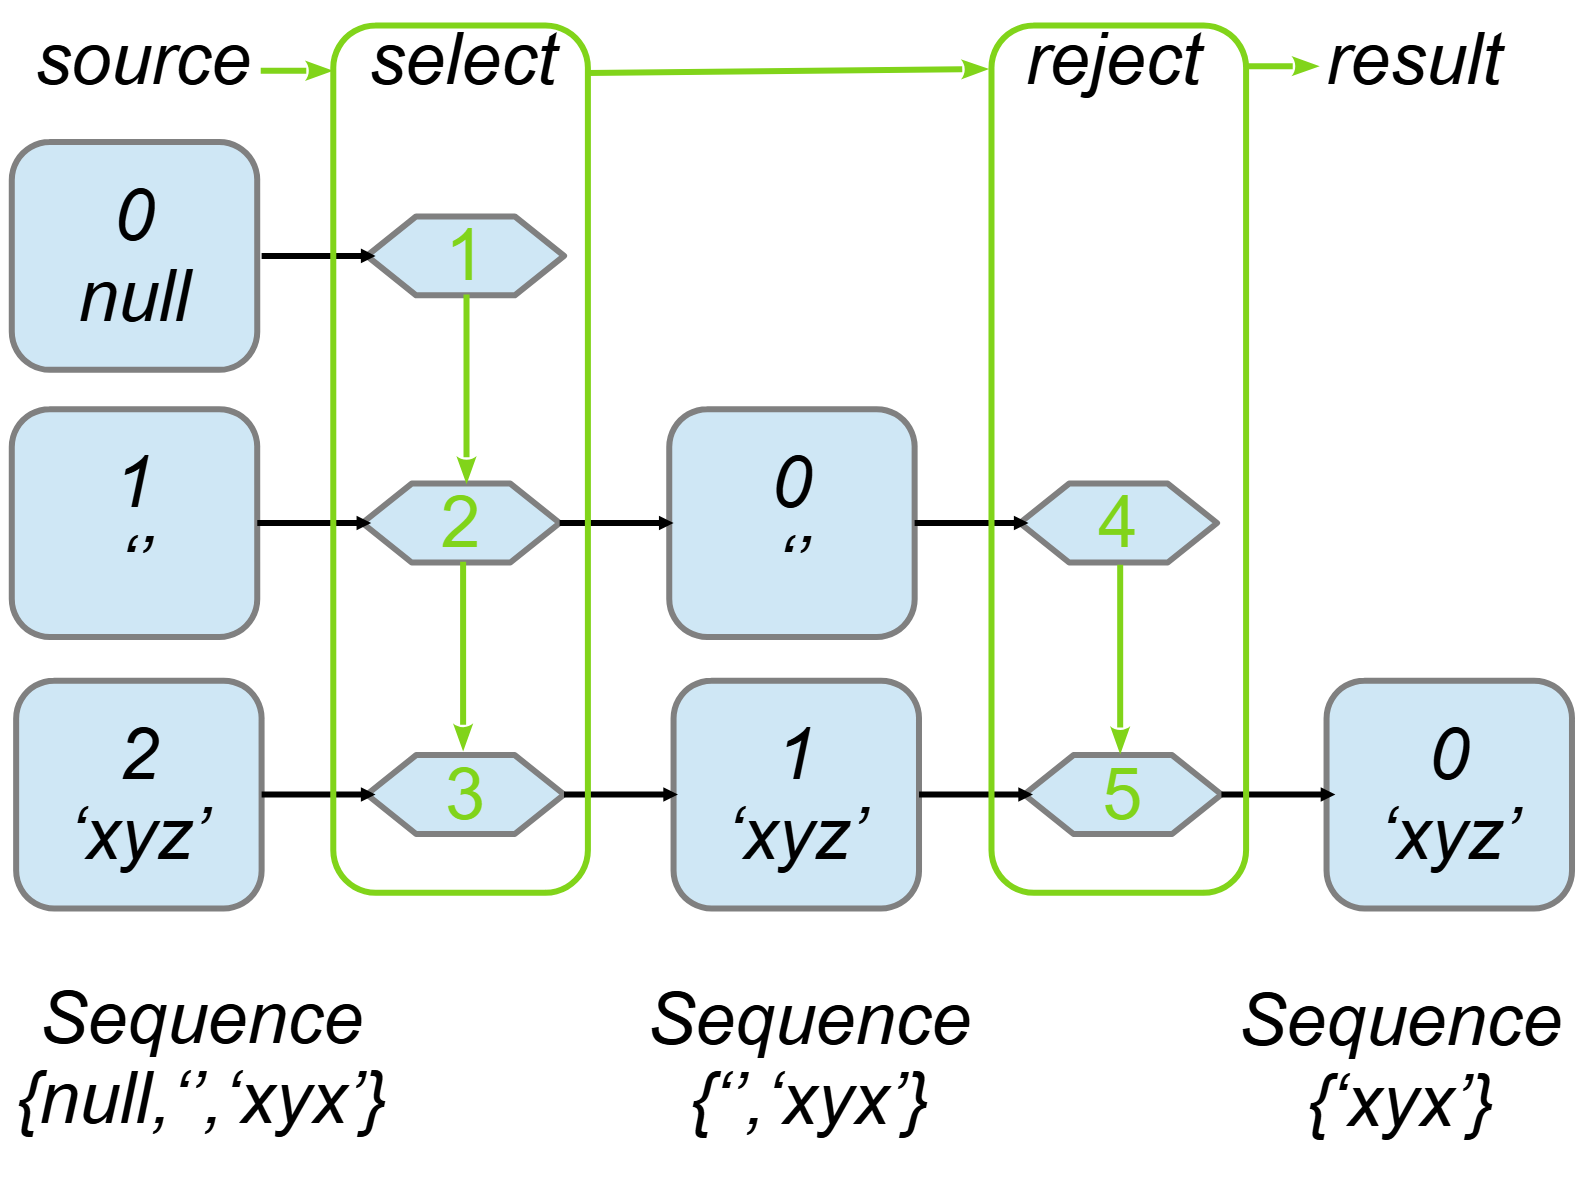
\includegraphics[width=5.0in]{ExampleStandard.png}
	\end{center}
	\vspace{-10pt}
	\caption{Simple Example (traditional approach)}
	\label{fig:ExampleStandard}
	\vspace{-10pt}
\end{figure}

The \verb!Sequence{null, '', 'xyz'}! \verb!source! value at left is passed to the \verb!select! iteration building block which processes each element in turn to produce the \verb!Sequence{'', 'xyz'}! intermediate result.  Control is then passed to the \verb!reject! iteration building block so that each element of the intermediate result is processed to produce the overall  \verb!Sequence{'xyz'}! \verb!result! at right. The vertical then horizontal order of evaluation is shown by green arrows and the 1..5 labels on the computation lozenges. This order of execution is very natural when an implementation is based on subroutines for each operation/iteration building block.

We would obviously like our execution to perform all the necessary computations while performing as few extra activities as possible. The processing in Fig~\ref{fig:ExampleStandard} does not satisfy this desire. Each execution of \verb!name <> null! and \verb!name = ''! is clearly necessary, as is access to the \verb!source!, and assignment of the \verb!result!. But almost everything else is questionable bloat.

The execution creates an unnecessary intermediate result and traverses two collections for many of the result elements. (Worse, if the intermediates and results are maintained as OCL collections, an unnecessary OCL collection is churned for each iteration step; a fresh collection is successively created for  \verb!Sequence{}! and then \verb!Sequence{''}! before the useful \verb!Sequence{'','xyz'}! intermediate is passed.

\subsection{Faster Execution Flow}

It is intuitively obvious that our example could be rewritten as

\begin{description}[itemsep=-0.2cm]\small
\item ~~~~\verb!source->select((name <> null) and not (name = ''))!
\end{description}

Figure~\ref{fig:ExampleIntutive} shows the correspondingly better horizontal then vertical execution. The intermediate passed between computations is a single element rather than a collection. This element is easily accommodated by a hardware register avoiding the need to allocate, populate and traverse memory for an intermediate collection. (The second execution lozenge is hatched out since it has nothing to process.)

\begin{figure}
	\vspace{-10pt}
	\begin{center}
%		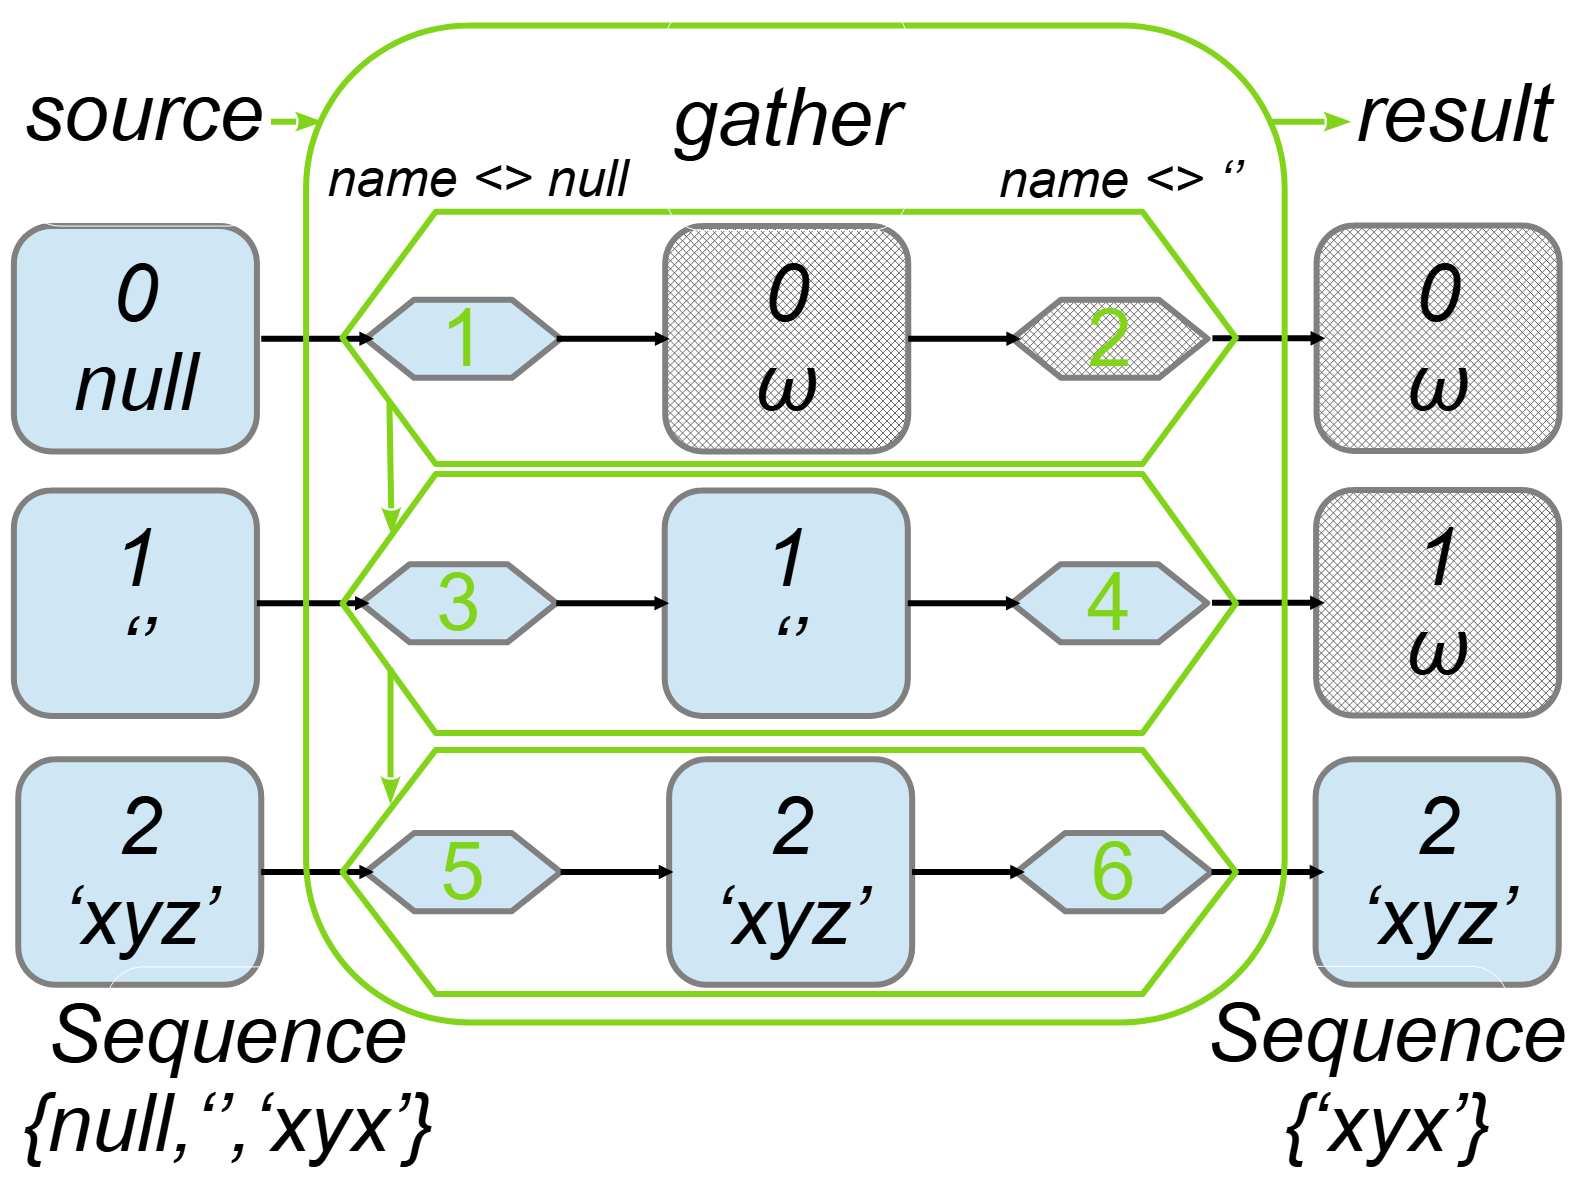
\includegraphics[trim={0 5cm 1cm 0},clip,width=6.0in]{ExampleImproved.jpg}
		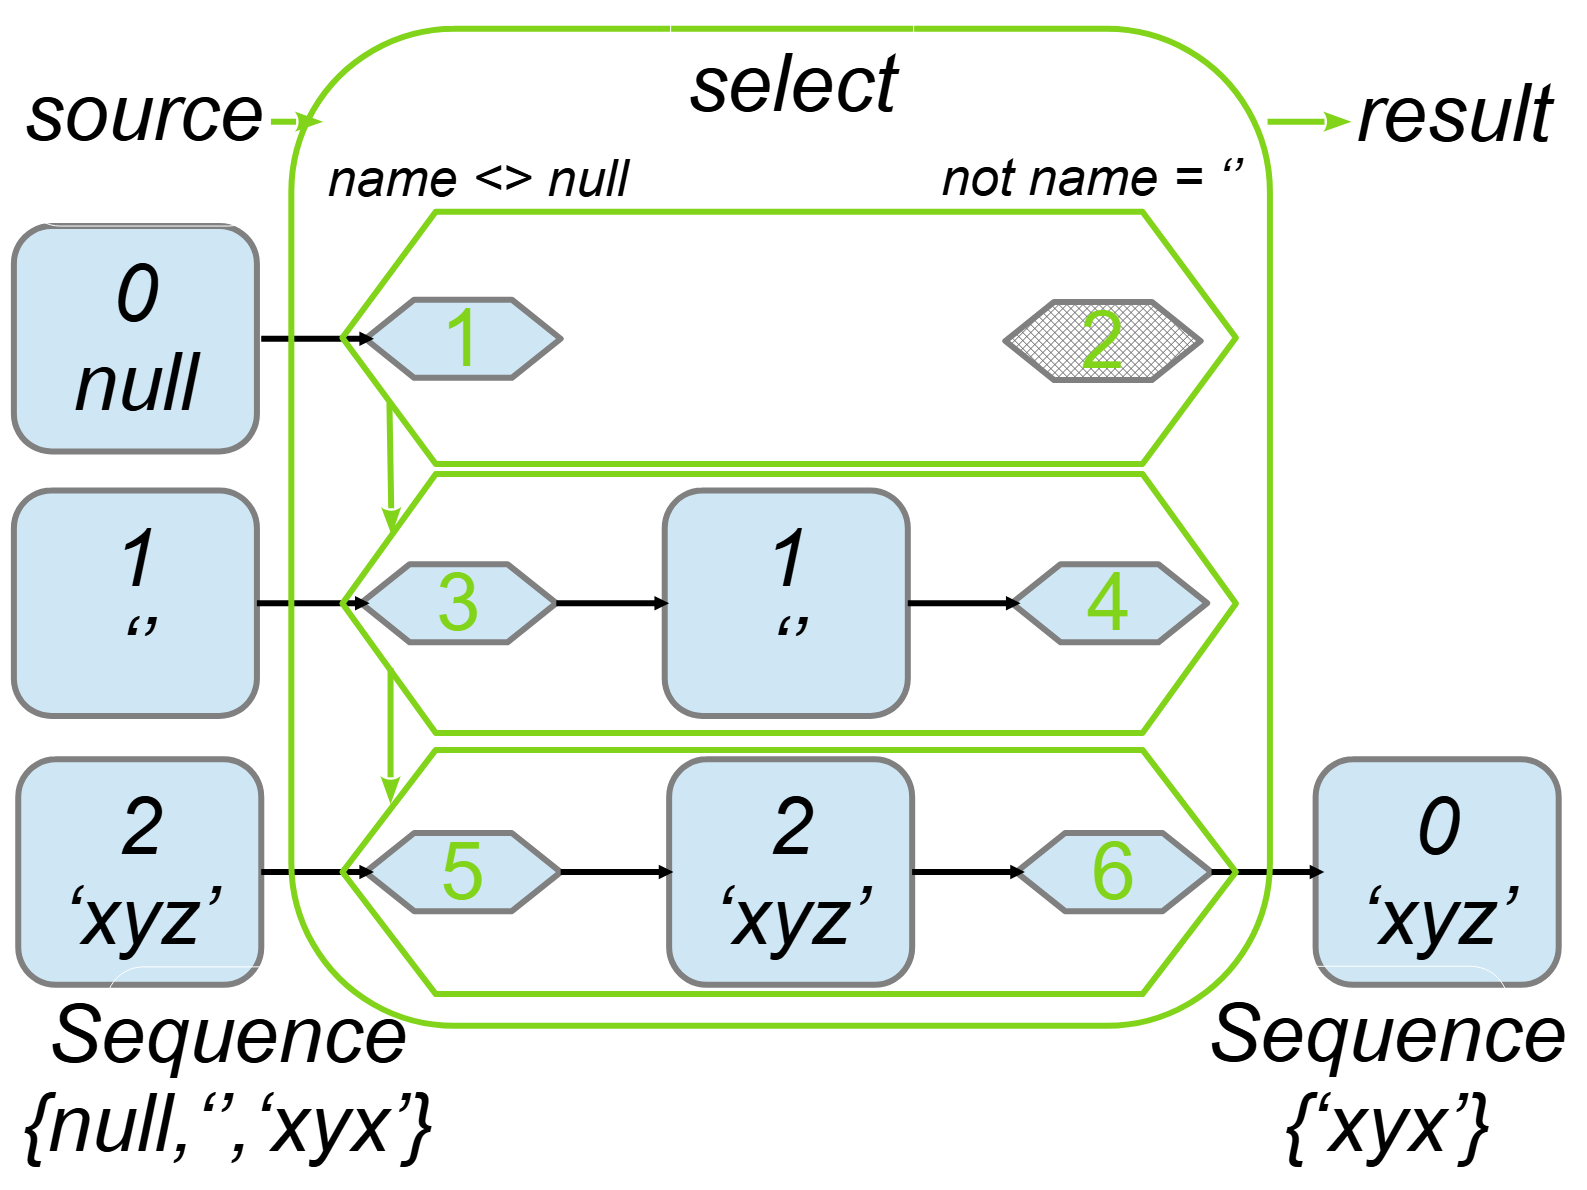
\includegraphics[width=6.0in]{ExampleIntuitive.png}
	\end{center}
	\vspace{-10pt}
	\caption{Simple Example (intuitive approach)}
	\label{fig:ExampleIntutive}
	\vspace{-10pt}
\end{figure}

However the OCL specification provides no formality for this intuition. It is debatable whether the single-select rewrite is more readable, so it is unreasonable to expect an OCL author to write in this tooling-friendly rather than reader-friendly style. An efficient OCL tool should perform the rewrite automatically.

Recognition of \verb!select! followed by \verb!reject! could be characterized as a high level form of Peephole Optimization. With 10 distinct iterations and four distinct collection kinds we could require (4*10)*(4*10)=1600 candidate peephole optimizations to be assessed and coded for all possible 2-term permutations; yet more for 3-term. 

In the part 2 sister paper, we re-characterized collection operations and iterations using the new \verb!gather! and \verb!search! iterations. We will now use these to derive the intuitively obvious approach in a way that can be automated with no peephole optimizations for \verb!gather!. 

\subsection{gather-gather optimization}\label{gather-gather optimization}

The \verb!Sequence! overload of \verb!gather! is modeled using the Eclipse OCL standard library as:

\begin{description}[itemsep=-0.2cm]\small\begin{samepage}
\item ~~~~\verb!type Sequence(T) : SequenceType conformsTo OrderedCollection(T) {!
\item ~~~~\verb!{!
\item ~~~~~~~~\verb!iteration gather(V)(i : T[?] | lambda : Lambda T() : V[?]) : Sequence(V) {!
\item ~~~~~~~~~~~~\verb!post: self->forAll(i with x | result->at(x) = i.lambda());!
\item ~~~~~~~~\verb!}!
\item ~~~~~~~~\verb!iteration select(i : T[?] | lambda : Lambda T() : Boolean[1]) : Sequence(T) {!
\item ~~~~~~~~~~~~\verb!body: self->gather(i | if i.lambda() then i else! $\omega$ \verb!endif)->compact();!
\item ~~~~~~~~\verb!}!
\item ~~~~\verb!}!
\end{samepage}\end{description}

The collection class template parameter \verb!T! and operation template parameter \verb!V! define the type signature. \verb!gather! has a single iterator \verb!i! whose type corresponds to the source collection element type; it may be null. The iteration body is modeled as a lambda expression named \verb!lambda! and typed as a \verb!Lambda! from a \verb!T! source without parameters to a \verb!V! return that may be null. The iteration result is a \verb!Sequence(V)!.

%The postcondition uses the Eclipse OCL coValue extension for iterators. The \verb!with! keyword introduces the coValue \verb!x!, which is a secondary iterator whose value is \verb!self->indexOf(i)!\footnote{Not quite. For a non-unique sequence, indexOf returns the first index; the coVolue increases monotonically.}. The postcondition therefore specifies that the result is element-wise the result of computing the lambda expression for the input element.

The postcondition specifies that the result is element-wise the result of computing the lambda expression for the input element.

The specification of \verb!select! once again has a source-typed iterator \verb!i!, and a lambda-expression, that is now required to have a \verb!Boolean! result. The \verb!body! defines an implementation of the iteration that rewrites to the \verb!gather! iteration with a nested lambda-expression that wraps the selection. The OCL specification suggests that \verb!select! and other iterations can be realized by \verb!iterate!. This is inefficient since \verb!iterate!'s accumulator is procedural; the accumulator successively accumulates each result element, creating a new result collection at each step. In contrast, the rewrite to use \verb!gather! is declarative with the special value $\omega$ used as a placeholder for the not-available value on the dead computation path. The $\omega$ terms are squeezed out by the \verb!compact! operation.

This recharacterization supports the rewrite of our example (with explicit iterators):

\begin{description}[itemsep=-0.2cm]\small\begin{samepage}
\item ~~~~\verb!source->gather(i | if (i.name <> null) then i else! $\omega$ \verb!endif)!
\item ~~~~~~~~~~~~~~~~~~\verb!->compact()!
\item ~~~~~~~~~~~~~~~~~~\verb!->gather(j | if not j.name = '' then j else! $\omega$ \verb!endif)!
\item ~~~~~~~~~~~~~~~~~~\verb!->compact()!
\end{samepage}\end{description}

We may simplify the \verb!if! and eliminate the first \verb!compact! by handling the $\omega$ downstream.

\begin{description}[itemsep=-0.2cm]\small\begin{samepage}
\item ~~~~\verb!source->gather(i | if i.name <> null then i else! $\omega$ \verb!endif)!
\item ~~~~~~~~~~~~~~~~~\verb!->gather(j | if (j <>! $\omega$\verb!) and (not j.name = '') then j else! $\omega$ \verb!endif)!
\item ~~~~~~~~~~~~~~~~~\verb!->compact()!
\end{samepage}\end{description}

Both \verb!gather!s operate in lock-step element-wise with no dependency on sibling iterations, so we may merge the second into the first using the result of the first as the iterator of the second.

\begin{description}[itemsep=-0.2cm]\small\begin{samepage}
\item ~~~~\verb!source->gather(i |!
\item ~~~~~~~~~~~~~~~~~~~~~~~~~~~~\verb!let j = if i.name <> null then i else! $\omega$ \verb!endif in!
\item ~~~~~~~~~~~~~~~~~~~~~~~~~~~~\verb!if (j <>! $\omega$\verb!) and (not j.name = '') then j else! $\omega$ \verb!endif)!
\item ~~~~~~~~~~~~~~~~~\verb!->compact()!
\end{samepage}\end{description}

Substituting the let-variable for \verb!j! and simplifying gives:

\begin{description}[itemsep=-0.2cm]\small\begin{samepage}
\item ~~~~\verb!source->gather(i | if (i.name <> null) and (not i.name = '')!
\item ~~~~~~~~~~~~~~~~~~~~~~~~~~~~~~~~~~~~\verb!then i else! $\omega$ \verb!endif)!
\item ~~~~~~~~~~~~~~~~~\verb!->compact()!
\end{samepage}\end{description}

This provides a rational automate-able derivation of the intuitively obvious. %The \verb!gather!-\verb!gather! optimization is possible when the second \verb!gather! has no cross-dependencies on the intermediate results.

%Since the gathers are isomorphic  \verb!x! and  \verb!y! represent the same index.
%\begin{description}[itemsep=-0.2cm]\small
%\item ~~~~\verb!source->gather(name <> null)->gather(not name = '')->compact()!
%\end{description}

%\verb!gather! defines a per-element operation, so provided the later bodies, such as are \verb!not name = ''! are position and sibling independent, we may %merge the bodies. This provision is hard to violate since in the absence of a let variable to reify the intermediate, the later bodies cannot access the %intermediates and so their sibilings.

%\begin{description}[itemsep=-0.2cm]\small
%\item ~~~~\verb!source->gather((name <> null) and (not name = ''))->compact()!
%\end{description}

%\verb!gather! does not compact automatically. This ensures that the element indexes for the first iteration remain valid across the intermediates and result. 

The corresponding processing and control flow is shown in Fig~\ref{fig:ExampleImproved}. The  \verb!select! and  \verb!reject! are aggregated by the \verb!gather!. The compound processing for \verb!name <> null! and \verb!not (name = ''))! computations sequences `horizontally' rather than `vertically'. 
As well as the changed order of evaluation, Fig~\ref{fig:ExampleImproved} shows a hatched background with dead/not-available values represented as $\omega$.

There is now no unnecessary intermediate result and no need for two collection traversals. The comparative performance of alternate implementations of this example are presented in Section~\ref{Results}.

%When the compuations in Fig~\ref{fig:ExampleStandard} are independent of the collection index or other collection contents, there is an alternative computation flow. All the computations for the first element can be performed in turn followed by the computions for the next element and so forth as shown in Figure Y. This avoids the full collection intermediate flow. Only an intermediate collection element is required at typically no cost. Redrawing Fig~\ref{fig:ExampleStandard} as Fig~\ref{fig:ExampleImproved} so that the 'result' is isomorphic wrt the source. $\omega$ 'values' fill in the missing values and are stripped from the result before presenting it to a user. The isomorphism ensures that all stages of the computation have a constant index and so may re-use the source CoCollection. 

\begin{figure}
	\vspace{-10pt}
	\begin{center}
%		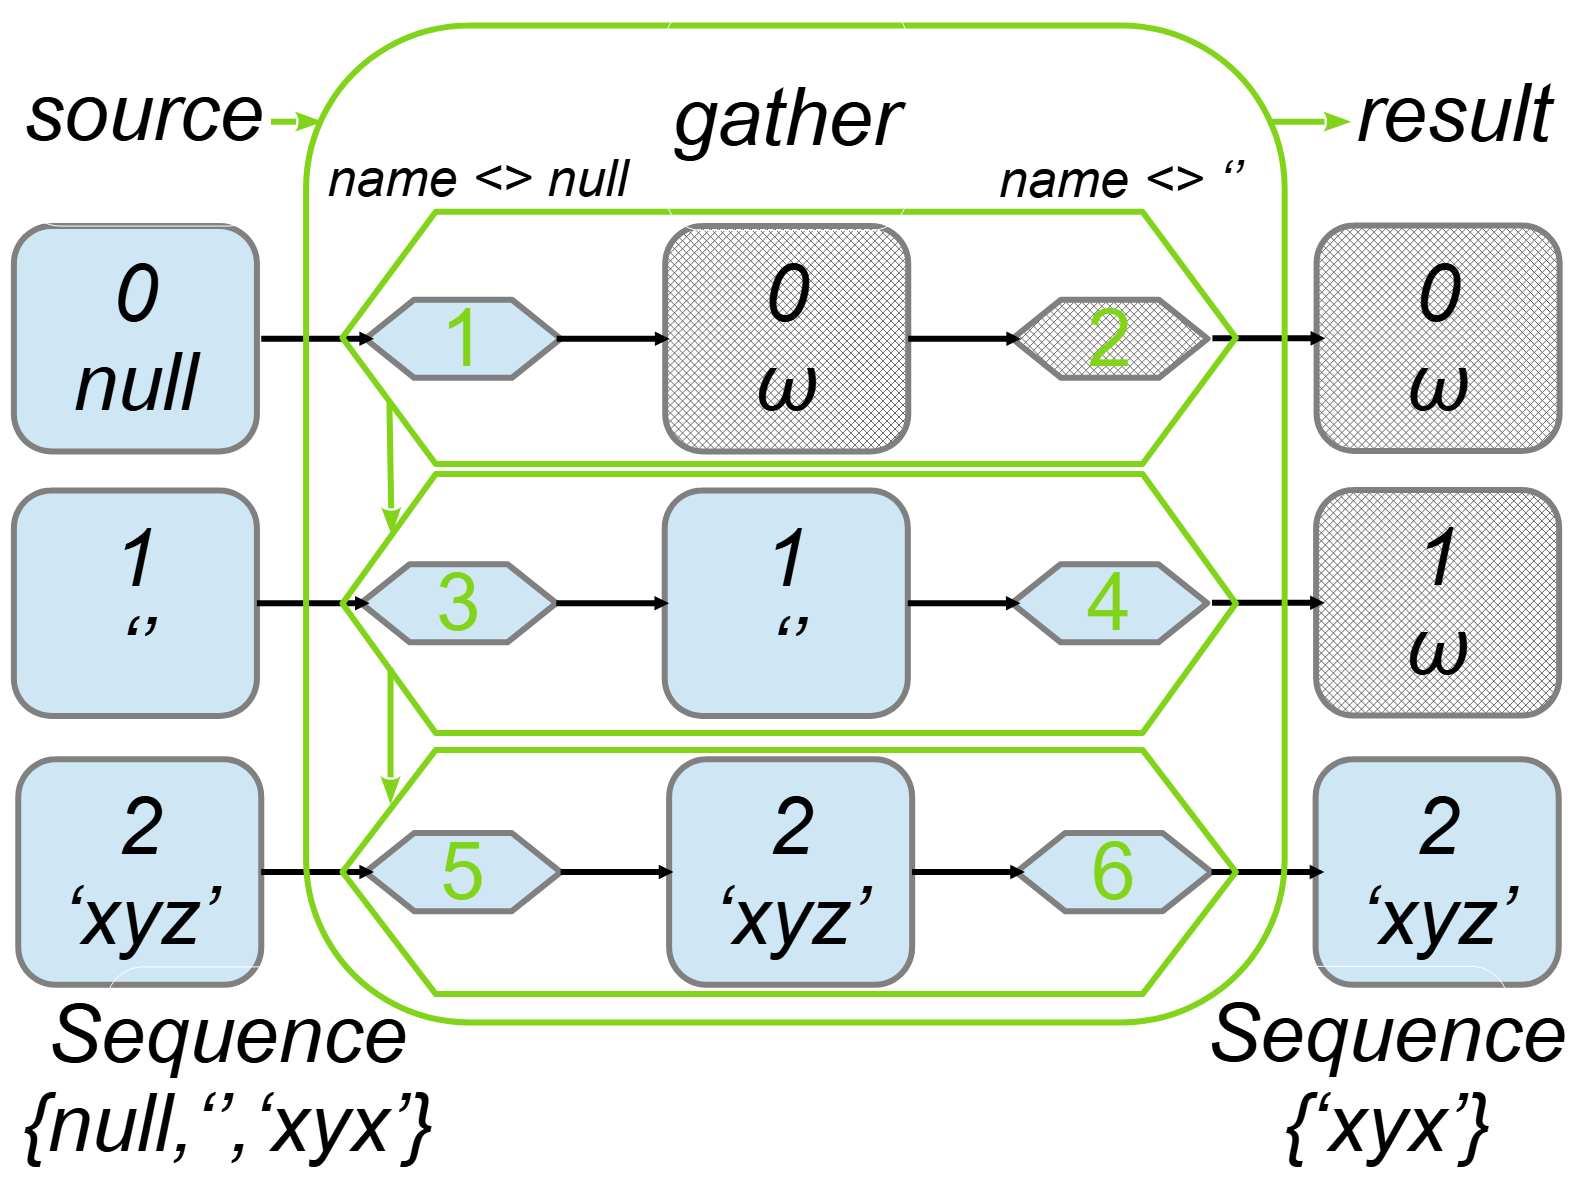
\includegraphics[trim={0 5cm 1cm 0},clip,width=6.0in]{ExampleImproved.jpg}
		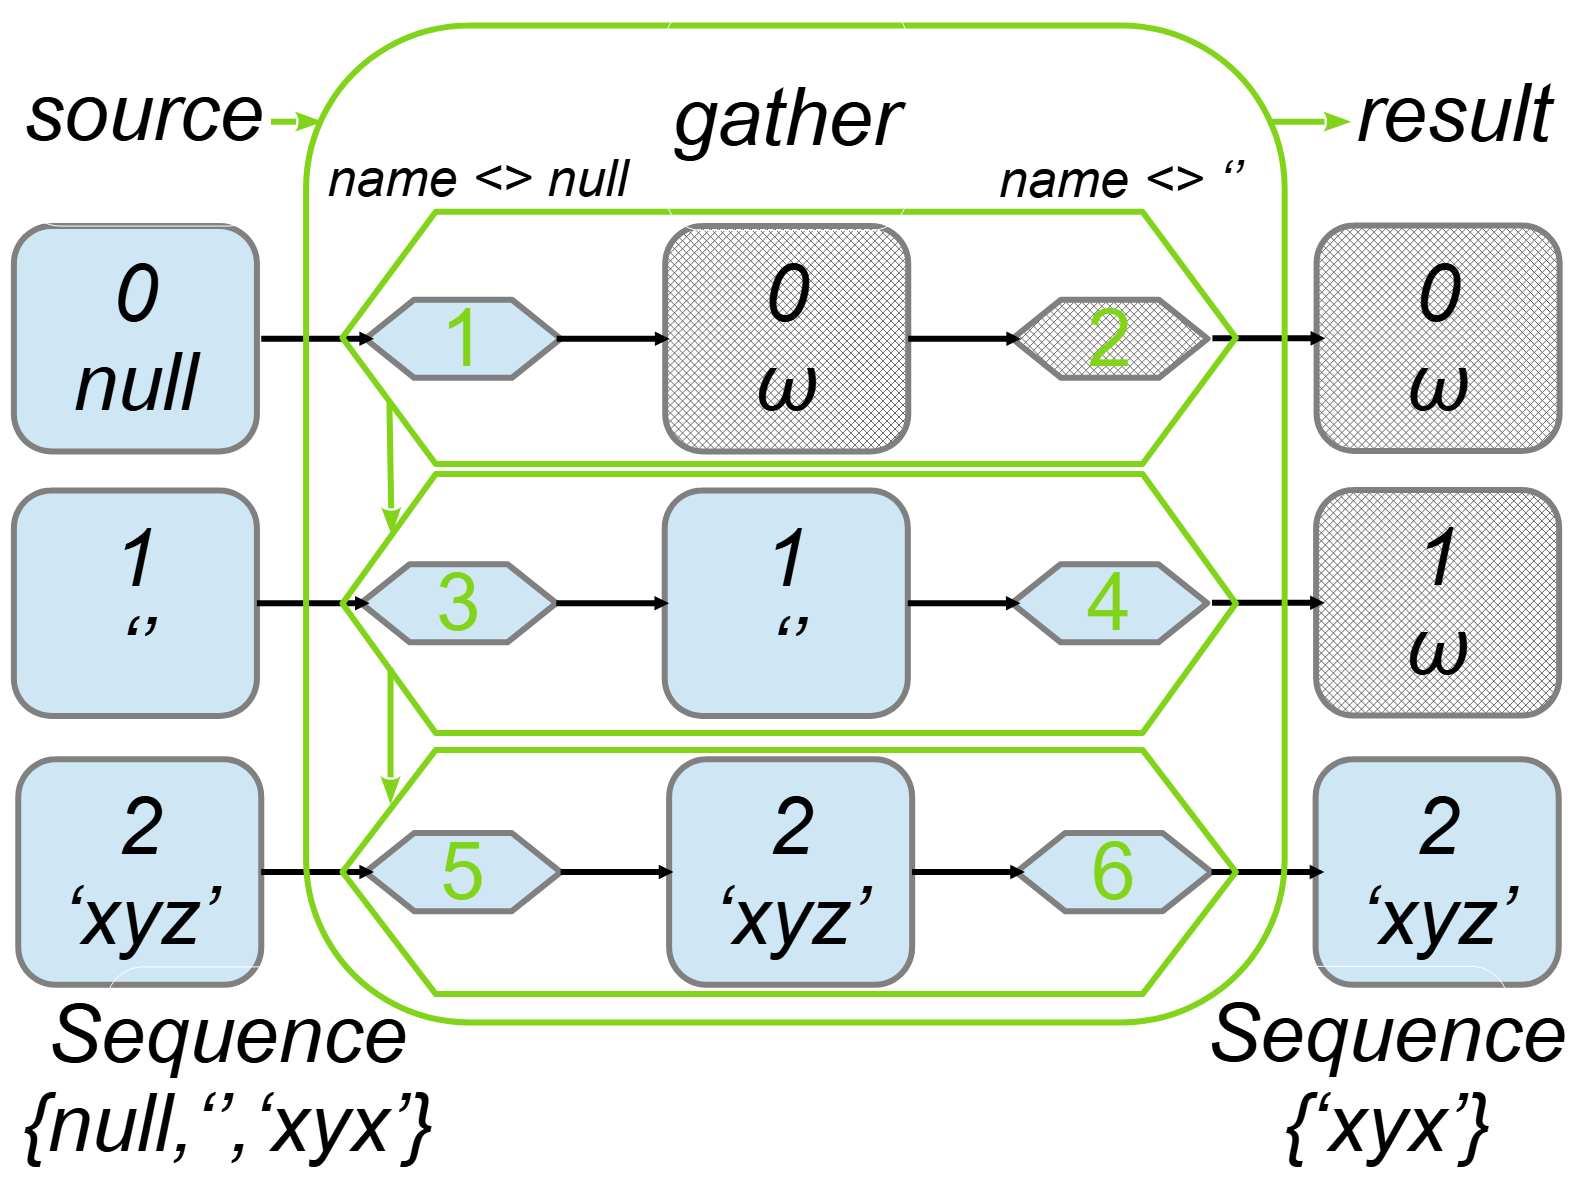
\includegraphics[width=6.0in]{ExampleImproved.png}
	\end{center}
	\vspace{-10pt}
	\caption{Simple Example (improved approach)}
	\label{fig:ExampleImproved}
	\vspace{-10pt}
\end{figure}

\subsection{gather-gather optimization for sets}

With many, perhaps all, declarative iterations and operations amenable to rewriting to use \verb!gather!, there will be many opportunities for \verb!gather!-\verb!gather! cascades to be identified and optimized.

However there is one major impediment to this optimization; the execution of each per-element lambda-expression must be mutually independent. This condition is not satisfied by set iterations over a non-set since each element execution must check that it is not duplicating an earlier execution. The simple solution is to reify the set between the \verb!gather!s, but that incurs the cost of creating the set.

The \verb!CoCollection! provides an alternative solution, which may often be faster and certainly smaller. The `uniqueness' is realized as a potentially one-bit per-element Boolean flag that indicates whether the element is the first element with the associated element value. This contrasts with at least 128 bits per element for a Java HashSet node. Use of a  \verb!CoCollection! supports the rewrite of set creation and then some collection operation as in \verb!x->asSet()->collectNested(...)! to use \verb!gather! as:

\begin{description}[itemsep=-0.2cm]\small\begin{samepage}
\item \verb!x->asSet()->gather(...)->compact()!
\end{samepage}\end{description}

The \verb!asSet! can be replaced by a \verb!coCollection.isFirst! guard.

\begin{description}[itemsep=-0.2cm]\small\begin{samepage}
\item \verb!let coCollection = x->coCollection() in!
\item ~~~~~~~~\verb!x->gather(i | if coCollection.isFirst(i) then ... else! $\omega$ \verb!endif)!
\item ~~~~~~~~~~\verb!->compact()!
\end{samepage}\end{description}

The element interdependence is now localized in the \verb!coCollection! for which the first invocation of \verb!isFirst! will trigger the lazy evaluation. The bodies of multiple \verb!gather!s involving sets can now be merged. However in practice data dependencies on the \verb!coCollection! may inhibit most merges. If one set is computed from another set, then obviously the first set is needed to avoid duplication.

There may however be a trade-off when the cost of duplication is low. Rather than de-duplicating immediately, it may be more efficient to perform duplicate calculations and de-duplicate later. This may well be worthwhile if the duplicated lambda-expressions are simple. It may also be worthwhile if the overall calculation may terminate early. It is then desirable to favor maximizing horizontal progress to discover an early termination over eager vertical determination of uniqueness. A compiler can estimate the cost of the two approaches and generate code accordingly.

\section{Idioms}\label{Idioms}

Analysis of the UML 2.5 OCL constraints reveals a few idioms that are easily accommodated.

\subsection{selectByKind}

OCL 2.4 introduced the \verb!x->selectByKind(T)! operation to replace the clumsy \verb!x->select(oclIsKindOf(T))->collect(oclAsType(T))!. However at least 10 usages for UML 2.5 remain. These are automatically resolved by successive rewrites to 

\begin{description}[itemsep=-0.2cm]\small\begin{samepage}
\item  ~~~~\verb!x->gather(p | if p.oclIsKindOf(T) then p else!~\(\omega\)~\verb!endif)!
\item  ~~~~~~~\verb!->compact()!
\item  ~~~~~~~\verb!->gather(oclAsType(T))!
\item  ~~~~~~~\verb!->compact()!
\end{samepage}\end{description}
\begin{description}[itemsep=-0.2cm]\small\begin{samepage}
\item  ~~~~\verb!x->gather(p | if p.oclIsKindOf(T) then p else!~\(\omega\)~\verb!endif.oclAsType(T))!
\item  ~~~~~~~\verb!->compact()!
\end{samepage}\end{description}
\begin{description}[itemsep=-0.2cm]\small\begin{samepage}
\item  ~~~~\verb!x->gather(p | if p.oclIsKindOf(T) then p.oclAsType(T) else!~\(\omega\)~\verb!endif)!
\item  ~~~~~~~\verb!->compact()!
\end{samepage}\end{description}

The final \verb!p.oclAsType(T)! is necessary to ensure that \verb!T! is seen by downstream expressions. It is not necessary when executing, since the preceding \verb!p.oclIsKindOf(T)! guarantees that it is a no-op. The rewrite to \verb!x->gather(...)->compact()! gives the same result as \verb!selectByKind(...)!. Execution of the \verb!gather(...)! can of course compact as it goes rather than produce a bloated intermediate that is then compacted.

Normalization to use  \verb!gather! renders \verb!selectByKind! redundant, although the user may nonetheless choose to use \verb!selectByKind! for readability.

\subsection{select-then-count}
Another common idom in the UML 2.5 OCL constraints is epitomized by

\begin{description}[itemsep=-0.2cm]\small\begin{samepage}
\item ~~~~\verb!behavior.ownedParameter->select((direction =!
\item ~~~~~~~~\verb!UML::Classification::ParameterDirectionKind::return))->size() = 1!
\end{samepage}\end{description}

This could have used the \verb!one()! iteration. Similarly

\begin{description}[itemsep=-0.2cm]\small
\item ~~~~\verb!allNamespaces()->select(ns | (ns.name = null))->notEmpty()!
\end{description}

could have used the \verb!exists()! iteration. However

\begin{description}[itemsep=-0.2cm]\small
\item ~~~~\verb!parameterSubstitution->select(b | (b.formal = p))->size() <= 1!
\end{description}
has no shorter form.

These examples all demonstrate a common theme; a computation to count rather than use the results. 

We can rewrite \verb!size! using a \verb!search! for use when following a \verb!gather! so let us investigate the \verb!gather!-\verb!search! optimization.

\section{gather-search optimization}\label{gather-search-optimization}

We have described the \verb!compact! operation, but not defined it. With the aid of the new \verb!search! iteration we can define it together with helpful variants. The definition of these is modeled as follows.

\begin{description}[itemsep=-0.2cm]\small\begin{samepage}
\item ~~~~\verb!type Sequence(T) : SequenceType conformsTo OrderedCollection(T)!
\item ~~~~\verb!{!
\item ~~~~~~~~\verb!iteration search(V,W)(i : T[?]; !
\item ~~~~~~~~~~~~~~~~~~~~~~~~~~~~~~~~~~~~~~~~~~~~~~~~~~~~~~~~\verb!acc : W |!
\item ~~~~~~~~~~~~~~~~~~~~~~~~~~~~~~~~~~~~~~~~~~~~~~~~~~~~~~~~\verb!next : Lambda T() : W,!
\item ~~~~~~~~~~~~~~~~~~~~~~~~~~~~~~~~~~~~~~~~~~~~~~~~~~~~~~~~\verb!break : Lambda T() : Boolean,!
\item ~~~~~~~~~~~~~~~~~~~~~~~~~~~~~~~~~~~~~~~~~~~~~~~~~~~~~~~~\verb!return : Lambda T() : V[?]) : V[?];!
\item ~~~~~~~~~~~~~~~~~~~~~~~~~~~~~~~~~~~~~~~~~~~~~~~~~~~~~~~\verb!) : V[?];!
\end{samepage}\end{description}
\begin{description}[itemsep=-0.2cm]\small\begin{samepage}
\item ~~~~~~~~\verb!operation compact() : Sequence(T) {!
\item ~~~~~~~~~~~~\verb!body: self->search(i; acc : Sequence(T) = Sequence{} |!
\item ~~~~~~~~~~~~~~~~~~~~~~~~~~~~~~~~~~~~~~~~~~~~\verb!if i =! $\omega$ \verb! then acc else acc->append(i) endif,!
\item ~~~~~~~~~~~~~~~~~~~~~~~~~~~~~~~~~~~~~~~~~~~~\verb!false, acc);!
\item ~~~~~~~~\verb!}!
\end{samepage}\end{description}
\begin{description}[itemsep=-0.2cm]\small\begin{samepage}
\item ~~~~~~~~\verb!operation compactingSize() : Integer {!
\item ~~~~~~~~~~~~\verb!body: self->search(i; size : Integer = 0 |!
\item ~~~~~~~~~~~~~~~~~~~~~~~~~~~~~~~~~~~~~~~~~~~~\verb!if i =! $\omega$ \verb! then size else size+1 endif,!
\item ~~~~~~~~~~~~~~~~~~~~~~~~~~~~~~~~~~~~~~~~~~~~\verb!false, size);!
\item ~~~~~~~~\verb!}!\end{samepage}\end{description}
\begin{description}[itemsep=-0.2cm]\small\begin{samepage}
\item ~~~~~~~~\verb!operation compactingSizeLessThan(sizeThreshold : Integer) : Boolean {!
\item ~~~~~~~~~~~~\verb!body: self->search(i; size : Integer = 0 |!
\item ~~~~~~~~~~~~~~~~~~~~~~~~~~~~~~~~~~~~~~~~~~~~\verb!if i =! $\omega$ \verb! then size else size+1 endif,!
\item ~~~~~~~~~~~~~~~~~~~~~~~~~~~~~~~~~~~~~~~~~~~~\verb!size >= sizeThreshold, size < sizeThreshold);!
\item ~~~~~~~~\verb!}!\item ~~~~\verb!}!
\end{samepage}\end{description}

The \verb!search! iteration like \verb!iterate! processes each input element sequentially with an iterator, accumulator and lambda-expression to determine the \verb!next! accumulator value. Syntactically they are separated by \verb!;! and then \verb!|!. \verb!iterate!'s limitations on early exit, and the requirement for the accumulator to be the result are removed by defining two further lambda-expression arguments. \verb!break! is true for the search to terminate early. \verb!return! is the value to be returned. To accommodate this flexibility, the outer class template parameter \verb!T! for the collection element type is augmented by the iteration template parameters \verb!V! and \verb!W! for result and accumulator types respectively.

The basic \verb!compact! operation appends non-$\omega$ inputs to create the output. It does not stop early.

Similarly the \verb!compactingSize! operation does not stop early. It counts rather than appends non-$\omega$ inputs to create the output. This avoids the need to create and repeatedly update a collection to accumulate unused results. 

The more powerful \verb!compactingSizeLessThan! also counts non-$\omega$ inputs, but breaks when \verb!size >= sizeThreshold! and returns \verb!size < sizeThreshold!. This not only avoids the unnecessary collection updates but also avoids unnecessary upstream computations.

A compiler optimizing

\begin{description}[itemsep=-0.2cm]\small
\item ~~~~~~~~\verb!x->select(...)->reject(...)->notEmpty()!
\end{description}

may initially rewrite as:

\begin{description}[itemsep=-0.2cm]\small
\item ~~~~~~~~\verb!x->gather(... and not ...)->compact()->notEmpty()!
\end{description}

then recognising the \verb!compact()->notEmpty()! idiom rewrite as

\begin{description}[itemsep=-0.2cm]\small
\item ~~~~~~~~\verb!x->gather(... and not ...)->compactingSizeNotEmpty()!
\end{description}

Finally rewriting the \verb!compactingSizeNotEmpty()! and merging the per-element bodies gives:

\begin{description}[itemsep=-0.2cm]\small
\item ~~~~~~~~\verb!x->search(i;  hasElement : Boolean = false |!
\item ~~~~~~~~~~~~~~~~\verb!if  ... and not ... then true else hasElement endif,!
\item ~~~~~~~~~~~~~~~~\verb!hasElement, hasElement)!
\end{description}

A cascade of declarative gathers can therefore be merged with a procedural search. Overall a single iteration is performed under control of the search.

In addition to the search iterations: 
\begin{description}[itemsep=-0.2cm]\small
\item ~~~~~~~~\verb!any!, \verb!exists!, \verb!forAll!, \verb!isUnique!, \verb!one!
\end{description}
the following OCL collection operations project a simple metric from a collection making reification of the collection unnecessary:
\begin{description}[itemsep=-0.2cm]\small
\item \verb!count!, \verb!excludes!, \verb!excludesAll!, \verb!includes!, \verb!includesAll!, \verb!isEmpty!, \verb!max!, \verb!min!, \verb!notEmpty!, \verb!size!, \verb!sum!
\end{description}

\subsection{search-search and search-gather optimization}

The \verb!search! iteration is procedural and often produces a single control value. There are therefore very limited prospects for collection optimizations following a \verb!search!.

%An OCL compiler has visibility of the full expression tree, which will usually permit all consumers of a intermediate result to be determined. The producer can therefore be notified of the aspects of the result that will be required.
The compacting phase of \verb!gather! can usefully be configured to count result terms rather than populate a redundant compacted result. And, when the absence of \verb!invalid! and \verb!null! is provable, the counting can terminate once a threshold has been passed.

\section{Results}\label{Results}

We can demonstrate the effect of good and bad implementation options with the rather extreme example of a \verb!HasValidlyNamedElement! constraint: 
\begin{description}[itemsep=-0.2cm]\small
\item \verb!x->select(name <> null)->reject(name = '')->notEmpty()!
\end{description}

Table \ref{tab:SelectRejectPerformance} shows the execution time for four different implementation options with model sizes varying from 10 to 1,000,000 model elements for \verb!x!. Each implementation is hand-coded in Java to demonstrate what an OCL to Java code generator might aspire to. The following pseudo-OCL defines each implementation using \verb!let...in...! to emphasize the intermediate variables of each implementation.

\begin{description}[itemsep=-0.2cm]\small\begin{samepage}
\item Set,Set ~~~~~~ \verb!let s1 = x->select(name <> null) in!
\item ~~~~~~~~~~~~~~~~~~ \verb!let s2 = s1->reject(name = '') in!
\item ~~~~~~~~~~~~~~~~~~ \verb!s2->size() > 0!
\item Set~~~~~~~~~~~~~ \verb!let s = x->select((name <> null) and not (name = '')) in!
\item ~~~~~~~~~~~~~~~~~~ \verb!s->size() > 0!
\item Count~~~~~~~~ \verb!x->iterate(e; acc : Integer = 0 |!
\item ~~~~~~~~~~~~~~~~~~~~~ \verb! if (name <> null) and not (name = '') then acc+1 else acc endif!
\item ~~~~~~~~~~~~~~~~~~~ \verb!) > 0!
\item Exists~~~~~~~ \verb! x->exists((name <> null) and not (name = ''))!
\end{samepage}\end{description}

The Set,Set implementation performs a \verb!select! followed by \verb!reject! followed by \verb!size! exactly as specified by the problem. A distinct set is created after each iteration.

The Set implementation merges the \verb!select! and \verb!reject! followed by \verb!size!. Only one set is created.

The Count implementation merges the \verb!select! and \verb!reject! and counts the results. No set is created.

The Exists implementation also merges the \verb!select! and \verb!reject! but breaks on the first valid name.

The results in Table \ref{tab:SelectRejectPerformance} show expected O(NlogN) trends where a set must be created and O(N) for the linear count. The Set result demonstrates the benefit of merging to perform a single \verb!select!. The Count result demonstrates the further benefit from just counting the per-element results. Finally the Exists result exploits a short circuit to terminate computation as soon as a definitive result is found.  

\begin{table}
\begin{tabular}{ c | c | c | c | c | c | c }
Components & 10 & 100 & 1000 & 10000 & 100000 & 1000000 \\
\hline
Set,Set & 0.000001 &  0.000006 &  0.000055 &  0.000565 &  0.014466 &  0.209042 \\
Set &  0.000000 &  0.000003 &  0.000023 &  0.000244 &  0.005122 &  0.067205 \\
Count &  0.000000 &  0.000000 &  0.000000 &  0.000002 &  0.000015 &  0.000188 \\
Exists &  0.000000 &  0.000000 &  0.000000 &  0.000000 &  0.000000 &  0.000000 \\
\end{tabular}
\caption{Select-Reject Example Performance in seconds}
\label{tab:SelectRejectPerformance}
\end{table}

The results are averaged over 100 runs to diminish the unpredictability caused by cache alignment fortuity. But perhaps 5\% randomness remains.%; the cost of the extra \verb!size! operation for Set,Set,Size compared to Set,Set should be swamped in comparison to the numerous element operations (the maximum and minimum ranges behind the average overlap.) %would not be expected to make any difference. The difference is due to a variety of causes. The speed of Set operations varies depending on the hashcodes and needs to rebalance the hash tree.  A first Set operation may be slowed if misses cause cache line thrashing. A later Set operation may be accelerated if the inputs to an earlier Set operation are still in the cache.. Further variation due to Java optimization is avoided by a substantial JVM warmup before taking measurements.

The important conclusions are as expected. Set computation is expensive\footnote{The Java HashSet is pretty good. Only slightly better performance is possible for smaller sets.}; two set operations are slower than one, one is slower than none. Avoiding unnecessary work by omitting unused results can be very beneficial.

%Our example to evaluate the benefits of more efficient cacscade processing is inspired on the \verb!Classification::Property::redefined_property_inherited! constraint:
%\begin{description}[itemsep=-0.2cm]\small
%\item ~~~~\verb!	redefinedProperty->notEmpty() implies (!
%\item ~~~~~~~~\verb!redefinitionContext->notEmpty() and!
%\item ~~~~~~~~\verb!redefinedProperty->forAll(rp |!
%\item ~~~~~~~~~~~~~~~~\verb!redefinitionContext!
%\item ~~~~~~~~~~~~~~~~~~~~~~~~\verb!->collect(fc | fc.allParents())!
%\item ~~~~~~~~~~~~~~~~~~~~~~~~\verb!->asSet()!
%\item ~~~~~~~~~~~~~~~~~~~~~~~~\verb!->collect(c | c.allFeatures())!
%\item ~~~~~~~~~~~~~~~~~~~~~~~~\verb!->asSet()!
%\item ~~~~~~~~~~~~~~~~~~~~~~~~\verb!->includes(rp)!
%\item ~~~~~~~~~~~~\verb!)!
%\item ~~~~\verb!	)!
%\end{description}

\section{Further Work}\label{Further Work}

The optimizations in this paper are very much a work in progress. Results demonstrating the promise of the approach are based on hand-coded Java; at the extremes the results demonstrate nearly 100\% and nearly 0\% optimization.. Considerable work is needed to integrate into Eclipse OCL. Only then can we discover the effectiveness of the optimizations on a large corpus such as the UML OCL constraints applied to a non-trivial model such as the UML metamodel.

\section{Related Work}\label{Related Work}

Cuadrado \cite{cuadrado2020verified} provides a catalog of OCL optimizations with the intent of tidying up the rather crazy OCL resulting from template-driven automated OCL synthesis. It is not expected that hand-written OCL would be improved. Most of the optimizations are subsumed by the symbolic Constant Folding and Common Subexpression Elimination of Eclipse OCL's Java Code Generator. Whereas Cuadrado attempts to inline let-expressions in the interest of `readability', Eclipse OCL's CSE maximizes let-variables so that partial results are amenable to Loop Hoisting. Many let-variables makes for a much simpler Java Code Generator avoiding complexities when an \verb!invalid! is thrown or caught within a complex expression. can be hoisted. Cuadrado's `iterators' optimizations are a form of peephole optimization subsumed by the more general \verb!gather!-\verb!gather! optimization presented in Section~\ref{gather-gather optimization}.

Cuadrado provides a comprehensive review of papers optimizing generation or rewriting of OCL. This paper seems to be unique in tunneling below the OCL specification to identify lower level primitives that improve performance.

\section{Summary}\label{Summary}

We have exploited the unification of the four collection kinds as a kind-specific views of a \verb!CoCollection! to reduce costs and share memory for diverse representations.

We have exploited the new declarative \verb!gather! and procedural \verb!search! iterations to normalize many collection operations and iterations by rewriting.

We have recognized that many results are just counted rather than used and so we define compacting variants to avoid creating the unused results.

With just one collection representation and two iteration representations, we are able to identify and optimize cascades of collection operations.

The effectiveness of the optimizations can vary from 0\% to 100\%. Future work will determine whether the optimizations are sufficient to make use of auto-generated code from OCL feasible for UML validation.


%% The declaration on generative AI comes in effect
%% in Janary 2025. See also
%% https://ceur-ws.org/GenAI/Policy.html
\section*{Declaration on Generative AI}
  The author(s) have not employed any Generative AI tools.


%%
%% Define the bibliography file to be used
\bibliography{OCLCollections}

\end{document}
